\chapter{Локальные квантовые поля и одномерное уравнение Дирака}

Мы уже познакомились с квантовыми полями через их кванты, операторы рождения и уничтожения и простейший гамильтониан для нерелятивистских частиц. Теперь мы заставим этот аппарат поработать. Сначала мы увидим, а не просто заявим, как пространственно-локальный гамильтониан сохраняет импульс. Затем мы позволим произведениям полей описывать рассеяние и распад и увидим, как многократное действие гамильтониана порождает зачатки диаграммной теории возмущений. Лишь после этого мы обратимся к обещанной проблеме фермионов. Самый ясный путь к ней — пока еще не фермионное поле, а одномерное уравнение Дирака.

\section{Гамильтониан поля еще раз}

Запишем гамильтониан для одного вида нерелятивистских частиц в виде
\begin{equation}
H_0=\int dx\,
\psi^\dagger(x)
\left[-\frac{\partial_x^2}{2m}+V(x)\right]
\psi(x).
\label{eq:l9-nonrel-hamiltonian}
\end{equation}
Обозначения выглядят одномерными, но в начальном рассуждении ничто не зависит от этого ограничения: в трех измерениях \(x\) может обозначать вектор \(\mathbf{x}\), \(dx\) — \(d^3x\), а \(-\partial_x^2\) — \(-\nabla^2\).

Оператор \(\psi^\dagger(x)\) создает частицу в точке \(x\), а \(\psi(x)\) уничтожает ее там. Их нормально упорядоченное произведение
\begin{equation}
n(x)=\psi^\dagger(x)\psi(x)
\end{equation}
есть локальная плотность числа частиц. Поэтому член с потенциалом имеет вид
\begin{equation}
H_V=\int dx\,V(x)n(x).
\end{equation}
Это в точности то, что мы записали бы для классического газа: подсчитать частицы вблизи \(x\), приписать каждой потенциальную энергию \(V(x)\) и просуммировать по пространству. На этом этапе частицы друг с другом не взаимодействуют. Они могут откликаться на внешне заданный потенциал, но в остальном гамильтониан представляет собой сумму независимых одночастичных энергий.

Полезно сначала упростить ситуацию, а затем пойти в обратную сторону. Пусть потенциал постоянен, \(V(x)=V_0\). Постоянный потенциал не создает силы, однако его операторный смысл прозрачен:
\begin{equation}
\begin{aligned}
H_V&=V_0\int dx\,\psi^\dagger(x)\psi(x)=V_0N,\\
N&=\int dx\,n(x).
\end{aligned}
\end{equation}
Он добавляет каждой частице одну и ту же добавку к энергии. Чтобы сохранить энергию покоя в нерелятивистском описании, выберем \(V_0=mc^2\). Тогда этот член учитывает по одной энергии покоя на каждую частицу. Мы сохраняем эту в остальном скучную константу, потому что она сохраняет трансляционную инвариантность и делает наглядной операцию счета частиц.

\section{Гамильтониан как правило обновления}

Что значит сказать, что импульс сохраняется? Ответ следует сформулировать через то, что делает гамильтониан. Чтобы не использовать \(\psi\) одновременно для полевого оператора, одночастичной волновой функции и многочастичного состояния, обозначим многочастичное состояние через \(\lvert\Phi(t)\rangle\). За короткий интервал \(\epsilon\),
\begin{equation}
\lvert\Phi(t+\epsilon)\rangle
=\left(1-i\epsilon H+O(\epsilon^2)\right)
\lvert\Phi(t)\rangle,
\label{eq:l9-short-update}
\end{equation}
где \(\hbar=1\). Неизменившееся состояние задается первым членом; первая поправка порождается \(H\). Итерация такого обновления и есть уравнение Schr\"odinger.

Теперь закон сохранения импульса приобретает конкретный смысл. Если начальное состояние имеет определенный полный импульс \(P\), то \(H\lvert\Phi\rangle\) должно иметь тот же полный импульс. Другие свойства могут изменяться, и отдельные частицы могут обмениваться импульсом, но гамильтониан не должен переводить состояние в сектор с другим полным \(P\). Это можно проверить напрямую, переписав гамильтониан в импульсном базисе.

\section{Пространственный интеграл как дельта-функция по импульсу}

Выберем соглашение для преобразования Фурье
\begin{align}
\psi(x)&=\int\frac{dp}{\sqrt{2\pi}}\,a(p)e^{ipx},\\
\psi^\dagger(x)&=\int\frac{dq}{\sqrt{2\pi}}\,a^\dagger(q)e^{-iqx}.
\label{eq:l9-field-fourier}
\end{align}
Оператор \(a(p)\) уничтожает частицу с импульсом \(p\).
Оператор \(a^\dagger(q)\) создает частицу с импульсом \(q\). Разные буквы существенны: оба импульса интегрируются независимо, пока пространственный интеграл не свяжет их.

Начнем с члена, отвечающего за число частиц:
\begin{align}
N
&=\int dx\,\psi^\dagger(x)\psi(x)\\
&=\int\frac{dp\,dq}{2\pi}\,
a^\dagger(q)a(p)
\int dx\,e^{i(p-q)x}.
\end{align}
Оставшийся интеграл равен
\begin{equation}
\int dx\,e^{i(p-q)x}=2\pi\delta(p-q).
\end{equation}
При \(p\ne q\) фаза осциллирует, и положительные и отрицательные вклады взаимно компенсируются. При \(p=q\) она вообще не осциллирует. Дельта-распределение Дирака — именно тот объект, который точно объединяет эти два факта. Следовательно,
\begin{align}
N
&=\int dp\,dq\,a^\dagger(q)a(p)\delta(p-q)\\
&=\int dp\,a^\dagger(p)a(p).
\label{eq:l9-number-momentum}
\end{align}
Оператор уничтожает частицу с импульсом \(p\) и создает взамен частицу в точности с тем же импульсом. Решающим элементом был интеграл по \(x\): он породил дельта-функцию, которая навязывает равенство входящего и исходящего импульсов.

\begin{classroomqa}
\lecturetimestamp{00:17:02}
\audiencequestion{Что произошло с бесконечностью, которая возникает при \(p=q\)?}
\lecturerresponse{Дельта-функцией пользуются не путем вычисления ее высоты. Это распределение, определяемое интегрированием: \(\int dk\,\delta(k)f(k)=f(0)\). Выражение ``бесконечно высокая и бесконечно узкая'' лишь напоминает, что ее интегральный вес равен единице. Здесь она велит нам положить \(p-q=0\), и никакого бесконечного ответа не остается.}
\end{classroomqa}

Тот же механизм работает и для гораздо более общего локального монома. Предположим, что некоторый член содержит несколько полей уничтожения и несколько полей рождения, возможно принадлежащих разным видам, но все они взяты в одной точке и проинтегрированы по этой точке:
\begin{equation}
\int dx\,
\prod_{r=1}^{n} \psi_{i_r}^\dagger(x)
\prod_{s=1}^{m} \psi_{j_s}(x).
\end{equation}
Пусть уничтожаемые частицы несут импульсы \(p_s\), а создаваемые — импульсы \(q_r\). Разложение Фурье дает
\begin{equation}
\int dx\,
e^{i(\sum_s p_s-\sum_r q_r)x}
=2\pi\,
\delta\!\left(\sum_s p_s-\sum_r q_r\right).
\label{eq:l9-total-momentum-delta}
\end{equation}
Результат не спаривает \(p_1\) с \(q_1\), \(p_2\) с \(q_2\) и так далее. Он налагает лишь условие
\begin{equation}
\sum_{\mathrm{annihilated}}p
=
\sum_{\mathrm{created}}q.
\end{equation}
Это именно то правило, которое требуется для взаимодействия: отдельные импульсы могут меняться, но полный импульс — нет. Более глубокое утверждение состоит в трансляционной инвариантности. Локальная плотность, проинтегрированная с одинаковым весом в каждой точке, не имеет выделенного начала отсчета, и ее преобразование Фурье несет соответствующую дельта-функцию, обеспечивающую сохранение импульса.

\begin{classroomqa}
\lecturetimestamp{00:23:04}
\audiencequestion{Предлагаемый член гамильтониана действительно является произведением всех этих полевых операторов? Почему мы вообще должны писать такое произведение?}
\lecturerresponse{Да. Это произведение задает, какие частицы уничтожаются и какие создаются в одной точке. Его физическая мотивация будет исходить из наблюдаемых процессов рассеяния или распада; рассуждение об импульсе устанавливается сначала, чтобы затем такие взаимодействия можно было сразу считывать.}
\end{classroomqa}

\section{Кинетическая энергия в импульсном и координатном пространствах}

Теперь применим тот же аппарат к члену с производной. Производная действует на плоскую волну:
\begin{equation}
-\partial_x^2 e^{ipx}=p^2e^{ipx}.
\end{equation}
Поэтому
\begin{align}
H_{\mathrm{kin}}
&=\int dx\,\psi^\dagger(x)
\left(-\frac{\partial_x^2}{2m}\right)\psi(x)\\
&=\int dp\,\frac{p^2}{2m}\,a^\dagger(p)a(p).
\label{eq:l9-kinetic-momentum}
\end{align}
И здесь пространственный интеграл снова навязывает равенство входящего и исходящего импульсов. Новый множитель \(p^2/2m\) просто взвешивает число частиц в каждой импульсной моде кинетической энергией этой моды.

\begin{classroomqa}
\lecturetimestamp{00:24:46}
\audiencequestion{Разве при двукратном дифференцировании плоской волны не должен появляться минус?}
\lecturerresponse{Да, \(\partial_x^2e^{ipx}=-p^2e^{ipx}\). В гамильтониане уже содержится компенсирующий минус, так что \(-\partial_x^2\) имеет положительное собственное значение \(p^2\).}
\end{classroomqa}

\begin{classroomqa}
\lecturetimestamp{00:27:20}
\audiencequestion{Кинетическая энергия сохраняется только тогда, когда потенциал постоянен?}
\lecturerresponse{Да. Если потенциал не зависит от координаты, силы нет, и кинетическая энергия сохраняется отдельно. Во внешнем непостоянном потенциале кинетическая и потенциальная энергии могут обмениваться, тогда как полный гамильтониан остается сохраняющейся величиной, если у него нет явной зависимости от времени.}
\end{classroomqa}

\begin{classroomqa}
\lecturetimestamp{00:27:42}
\audiencequestion{Какова роль \(\psi^\dagger\psi\) в кинетическом гамильтониане, записанном в импульсном пространстве?}
\lecturerresponse{Это оператор счета. Произведение мод \(a^\dagger(p)a(p)\) подсчитывает частицы с импульсом \(p\), а множитель \(p^2/2m\) приписывает каждой из них соответствующую кинетическую энергию.}
\end{classroomqa}

Есть и второй способ увидеть неотрицательность. Однократное интегрирование по частям с пренебрежением граничным членом дает
\begin{align}
\int dx\,\psi^\dagger(-\partial_x^2)\psi
&=\int dx\,(\partial_x\psi^\dagger)(\partial_x\psi).
\label{eq:l9-positive-kinetic}
\end{align}
Для полей, достаточно быстро обращающихся в нуль на бесконечности, или при периодических граничных условиях, граничный вклад равен нулю. Результат имеет вид модуля в квадрате и неотрицателен. Он также демонстрирует структуру, типичную для теории поля: энергия содержит квадраты пространственных производных полей.

\section{Локальное контактное взаимодействие}

Теперь придадим произведениям полей физическую роль. Рассмотрим два вида частиц, которые мы будем называть электроном и протоном лишь затем, чтобы картина оставалась привычной. Пока что они намеренно фиктивны: обе описываются бозонными операторами, а их настоящее кулоновское взаимодействие опущено. Их свободный гамильтониан имеет вид
\begin{equation}
H_0=\int dx\left[
\psi_e^\dagger\left(-\frac{\partial_x^2}{2m_e}\right)\psi_e
+
\psi_p^\dagger\left(-\frac{\partial_x^2}{2m_p}\right)\psi_p
\right].
\end{equation}
Добавим модельное взаимодействие
\begin{equation}
H_{\mathrm{contact}}
=g\int dx\,
\psi_e^\dagger(x)\psi_p^\dagger(x)
\psi_e(x)\psi_p(x).
\label{eq:l9-contact}
\end{equation}
Читайте это выражение справа налево. Оно ищет электрон и протон в одной и той же точке \(x\), уничтожает их и вновь создает обоих в той же точке. Если эти две частицы не находятся вместе, этот локальный член дает нуль. Если их мировые линии встречаются, он может изменить их индивидуальные импульсы, сохраняя полный. Тем самым он действует как идеализованный потенциал рассеяния нулевого радиуса действия.

\begin{figure}[htbp]
\centering
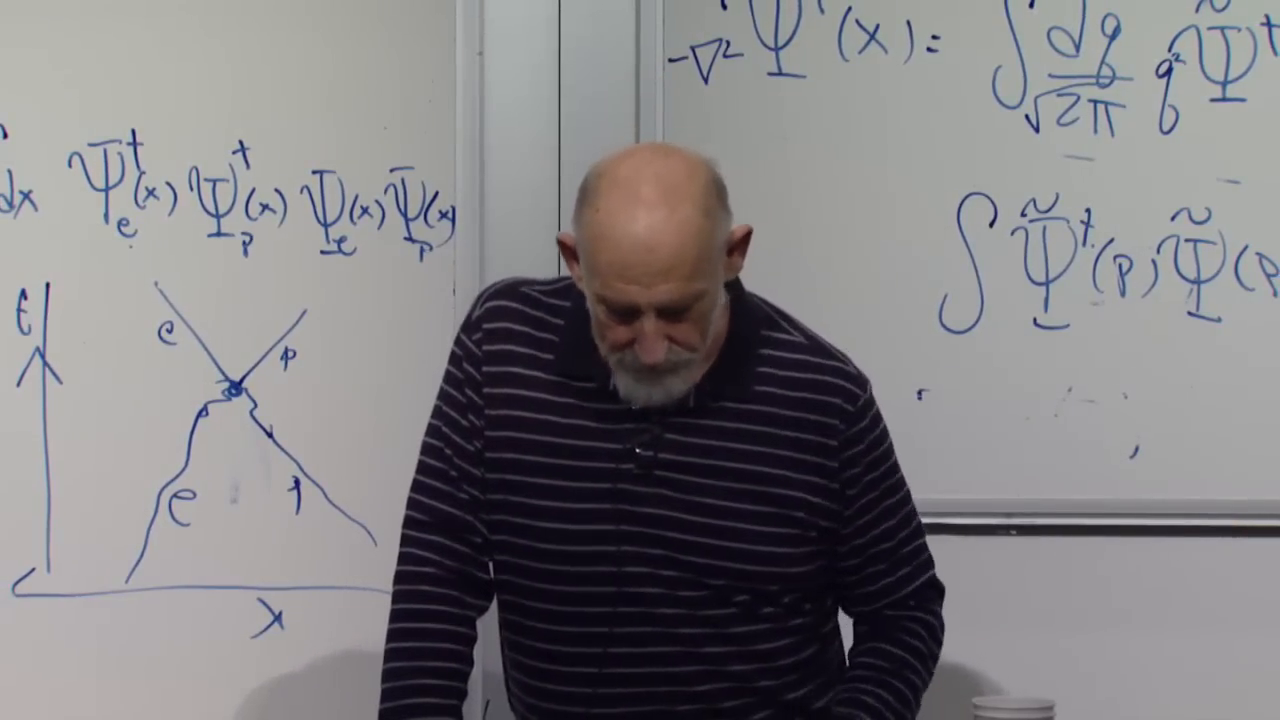
\includegraphics[width=0.94\linewidth]{lecture_09_frame_02.png}
\caption{Контактное взаимодействие на доске. Четыре локальных полевых оператора показаны над пространственно-временной схемой; точка встречи — единственное место, где действует идеализованное взаимодействие.}
\lectureframe{00:35:36}
\end{figure}

\begin{figure}[htbp]
\centering
\begin{tikzpicture}[x=1.2cm,y=1.0cm,>=Latex]
\draw[->] (-3.0,0) -- (3.0,0) node[right] {$x$};
\draw[->] (0,-0.2) -- (0,4.2) node[above] {$t$};
\coordinate (v) at (0,2.0);
\fill (v) circle (1.8pt);
\draw[thick,->] (-2.2,0.4) -- (v);
\draw[thick,->] (2.0,0.4) -- (v);
\draw[thick,->] (v) -- (-1.6,3.7);
\draw[thick,->] (v) -- (2.2,3.7);
\node[left] at (-1.65,0.7) {$e$};
\node[right] at (1.55,0.7) {$p$};
\node[left] at (-1.15,3.3) {$e$};
\node[right] at (1.65,3.3) {$p$};
\node[right] at (0.12,2.05) {$g$};
\end{tikzpicture}
\caption{Четкая реконструкция картины локального рассеяния. Вершина — это сокращенное обозначение оператора в уравнении~\eqref{eq:l9-contact}, а не классический закон столкновения.}
\end{figure}

Реальные электроны и протоны взаимодействуют на расстоянии через кулоновский потенциал. Контактная модель — лишь первый небольшой шаг: если бы эксперимент показал, что два вида частиц рассеиваются только при перекрытии, то в гамильтониан мы включили бы член вида ~\eqref{eq:l9-contact}.

\begin{classroomqa}
\lecturetimestamp{00:35:40}
\audiencequestion{Почему этот оператор рассеяния входит в гамильтониан, если энергия не меняется?}
\lecturerresponse{Гамильтониан — это и оператор энергии, и генератор, изменяющий состояние. Потенциальная энергия взаимодействия между двумя частицами порождает рассеяние при эволюции во времени. Сохранение полной энергии не означает, что состояние или отдельные импульсы частиц остаются неизменными.}
\end{classroomqa}

Это дает практическое правило. Сначала выясните из эксперимента, каким локальным процессам могут подвергаться частицы. Затем закодируйте эти процессы в операторе, который изменяет состояние. Произведения полей — не декоративная алгебра: множители с даггером и без него задают, какие виды частиц появляются и исчезают.

\section{Распад, обратный процесс и эрмитовость}

Предположим, что пузырьковая камера обнаруживает трек частицы вида \(A\), оканчивающийся в точке, из которой выходят треки \(B\) и \(C\). Локальный процесс имеет вид
\begin{equation}
A\longrightarrow B+C.
\end{equation}
Оператор, который его осуществляет, имеет вид
\begin{equation}
V=g\int dx\,
\psi_B^\dagger(x)\psi_C^\dagger(x)\psi_A(x).
\label{eq:l9-decay-half}
\end{equation}
Поле уничтожения уничтожает \(A\); два поля рождения создают \(B\) и \(C\) в одной и той же точке. Интегрирование с одинаковым весом по всем \(x\) выражает инвариантность относительно пространственных трансляций и сразу дает
\begin{equation}
p_A=p_B+p_C.
\end{equation}

Гамильтониан должен быть эрмитовым. Именно это делает \(e^{-itH}\) унитарным и обеспечивает сохранение полной вероятности. Выражение ~\eqref{eq:l9-decay-half} само по себе неэрмитово, поэтому мы должны добавить к нему эрмитово-сопряженный член:
\begin{equation}
H_{\mathrm{int}}
=\int dx\left[
g\,\psi_B^\dagger\psi_C^\dagger\psi_A
+g^*\,\psi_A^\dagger\psi_C\psi_B
\right](x).
\label{eq:l9-hermitian-vertex}
\end{equation}
Для вещественной константы связи \(g\) оба коэффициента совпадают. Эрмитово сопряжение не только заменяет поля с даггером на поля без него и наоборот, но и обращает порядок операторов. В этой игрушечной бозонной модели поля разных видов коммутируют, так что такое обращение не вызывает дополнительных осложнений.

Второй член осуществляет обратный процесс,
\begin{equation}
B+C\longrightarrow A.
\end{equation}
Следовательно, унитарный гамильтониан замкнутой системы, допускающий распад, также содержит амплитуду рекомбинации. Это не обещает, что оба направления реализуются для любого выбранного набора внешних импульсов; законы сохранения энергии и других величин могут сделать одно из направлений кинематически недоступным. Это означает, что и оператор, и его эрмитово-сопряженный член входят в динамику.

\begin{classroomqa}
\lecturetimestamp{00:42:48}
\audiencequestion{Может ли быть исключение из правила, что обратный процесс тоже разрешен?}
\lecturerresponse{Не на уровне эрмитова гамильтониана замкнутой системы: сопряженное взаимодействие обязательно. Конкретная обратная реакция все же может быть запрещена кинематикой или другим сохраняющимся квантовым числом, но сопряженный матричный элемент присутствует.}
\end{classroomqa}

Величина \(g\) — это константа связи. Если \(g\) мало, то встретившиеся частицы взаимодействуют лишь слабо; если оно велико, амплитуда перехода больше. Константы связи обычно являются параметрами, измеряемыми в экспериментах, хотя симметрии могут связывать несколько на вид различных констант связи.

Та же грамматика применима и к более сложным реакциям. В бета-распаде,
\begin{equation}
n\longrightarrow p+e^-+\bar\nu_e,
\end{equation}
схематический локальный член содержит четыре поля: одно уничтожает нейтрон, а три создают протон, электрон и электронное антинейтрино, вместе с эрмитово-сопряженным процессом. Этого достаточно, чтобы увидеть, как небольшой набор операторных мономов начинает задавать квантовую теорию поля.

\section{Почему важен квадрат гамильтониана}

В формуле для малого времени \eqref{eq:l9-short-update} сохранялся только первый порядок по \(\epsilon\). Полное разложение имеет вид
\begin{equation}
e^{-i\epsilon H}
=1-i\epsilon H-\frac{\epsilon^2}{2}H^2
+\frac{i\epsilon^3}{3!}H^3+\cdots.
\label{eq:l9-exponential}
\end{equation}
Во втором порядке гамильтониан действует дважды. В этом состоит алгебраическое происхождение первых изображений составных процессов.

Для вершины \(A\leftrightarrow B+C\) одно действие может объединить \(B+C\) в \(A\), а второе — снова превратить этот \(A\) в \(B+C\):
\begin{equation}
B+C\longrightarrow A\longrightarrow B+C.
\label{eq:l9-bc-scattering}
\end{equation}
В итоге получается вклад в амплитуду рассеяния \(B+C\to B+C\). Промежуточное \(A\) не является дополнительным наблюдаемым событием; оно обозначает состояние, по которому ведется суммирование между двумя действиями взаимодействия.

\begin{classroomqa}
\lecturetimestamp{00:49:54}
\audiencequestion{Должно ли поле \(C\) в записанном произведении второго порядка стоять с даггером?}
\lecturerresponse{Да, порядок операторов должен соответствовать указанной последовательности. Первая вершина уничтожает \(B\) и \(C\) и создает \(A\); вторая уничтожает \(A\) и вновь создает \(B\) и \(C\). Правильная расстановка даггеров восстанавливает именно эту интерпретацию.}
\end{classroomqa}

\begin{figure}[htbp]
\centering
\includegraphics[width=0.94\linewidth]{lecture_09_frame_05.png}
\caption{Две ориентации элементарной вершины \(A\leftrightarrow B+C\) на доске. Их расположение рядом — наглядная сокращенная запись процесса второго порядка из ~\eqref{eq:l9-bc-scattering}.}
\lectureframe{00:48:56}
\end{figure}

Теперь добавим спектаторную частицу \(B\). Одно действие позволяет \(A\) испустить \(C\) и превратиться в \(B\); последующее действие позволяет этому \(C\) соединиться с исходным \(B\) и образовать \(A\). Внешние частицы снова имеют виды \(A+B\), но их импульсы могут измениться. Мы описываем это как рассеяние \(A\) и \(B\) за счет обмена \(C\).

\begin{figure}[htbp]
\centering
\includegraphics[width=0.94\linewidth]{lecture_09_frame_06.png}
\caption{Построение обменного процесса на доске. Правая диаграмма соединяет две элементарные вершины внутренней линией \(C\), тогда как внешние частицы \(A\) и \(B\) рассеиваются.}
\lectureframe{00:51:22}
\end{figure}

\begin{figure}[htbp]
\centering
\begin{tikzpicture}[x=1.1cm,y=1cm,>=Latex]
\draw[->] (-3.7,-0.2) -- (-3.7,4.2) node[above] {$t$};
\coordinate (v1) at (-0.9,1.25);
\coordinate (v2) at (0.9,2.95);
\fill (v1) circle (1.7pt);
\fill (v2) circle (1.7pt);
\draw[thick,->] (-2.6,0.2) -- (v1) node[midway,below left] {$A$};
\draw[thick,->] (2.6,0.2) -- (v2) node[midway,below right] {$B$};
\draw[thick,->] (v1) -- (-2.4,4.0) node[midway,left] {$B$};
\draw[thick,->] (v2) -- (2.5,4.0) node[midway,right] {$A$};
\draw[thick,->,dashed] (v1) -- (v2) node[midway,above left] {$C$};
\node[below] at (0,-0.05) {$A+B\rightarrow A+B$};
\end{tikzpicture}
\caption{Аккуратная реконструкция обмена \(C\). Каждая точка вносит один множитель \(g\), так что этот член второго порядка пропорционален \(g^2\).}
\end{figure}

Каждая локальная точка взаимодействия называется вершиной. Каждая вершина вносит множитель своей константы связи, так что вклад с двумя вершинами несет \(g^2\), с тремя вершинами — \(g^3\) и так далее. Поэтому один-единственный член в гамильтониане связывает большое семейство реакций. Эта экономность — одна из причин, почему квантовая теория поля столь мощна: малое число локальных взаимодействий организует огромный массив данных о рассеянии.

\begin{classroomqa}
\lecturetimestamp{00:53:14}
\audiencequestion{Как называется процесс \(A\to B+C\to A\)?}
\lecturerresponse{Это вклад в собственную энергию. Наблюдаемое \(A\) — не просто голое одночастичное базисное состояние; у взаимодействующего состояния есть также амплитуда для близких компонент \(B+C\). Рассеяние на нем может выявить эту одетую структуру.}
\end{classroomqa}

Квантовая электродинамика дает знакомый пример. Локальная электрон--фотонная вершина может уничтожить электрон, вновь создать электрон и создать фотон. Во втором порядке электрон может испустить фотон и затем снова его поглотить. Заманчиво рассказывать об этом как о маленьком фильме, но в строгом смысле это член в пертурбативном разложении. Физический электрон — это одетое состояние с компонентами, содержащими фотон.

Оценка, приведенная на лекции, что эта компонента составляет ``около одного процента'', указывает на масштаб, задаваемый постоянной тонкой структуры, \(\alpha_{\mathrm{em}}\simeq 1/137\). Точная вероятность фоковской компоненты с фотоном зависит от энергетического разрешения и от того, как определено взаимодействующее состояние; это не универсальное свойство изолированного электрона на уровне одного процента. Надежное утверждение состоит в том, что взаимодействие изменяет измеримую структуру электрона.

\section{Что диаграмма говорит и чего она не говорит}

Диаграммы — это вычислительная сокращенная запись степеней гамильтониана взаимодействия. Они не являются надежными классическими историями, в которых частица определенно совершает одно событие, а затем другое. Попытка заглянуть внутрь и решить, какая промежуточная альтернатива ``действительно произошла'', меняет эксперимент и разрушает когерентную сумму, как и в обычной квантовой интерференции.

\begin{classroomqa}
\lecturetimestamp{00:56:52}
\audiencequestion{Сохраняются ли и энергия, и импульс в первой вершине?}
\lecturerresponse{В выполненной здесь гамильтоновой конструкции на равных временах пространственный интеграл сразу дает дельта-функцию по импульсу. Никакой интеграл по времени для этой отдельной вставки еще не дал дельта-функции по энергии. Полная амплитуда рассеяния, инвариантная относительно трансляций по времени, сохраняет полную энергию, тогда как промежуточные линии не обязаны удовлетворять соотношению на массовой поверхности, которому подчиняются наблюдаемые частицы. В ковариантном языке диаграмм четырехимпульс сохраняется в каждой вершине, но внутренние частицы могут быть вне массовой поверхности.}
\end{classroomqa}

Кажущееся отсутствие энергии в наивной картине вершины — еще одно предупреждение не отбрасывать энергию взаимодействия. Полный гамильтониан — это нечто большее, чем сумма энергий свободных частиц. Если возникает путаница, вернитесь к ~\eqref{eq:l9-exponential}: картинка обозначает член в разложении унитарной временной эволюции. Полная техника диаграмм Фейнмана систематически задает упорядочение по времени, пропагаторы, интегрирования и симметрийные множители, но базовая физика начинается уже здесь.

Развернутый вопрос слишком буквально трактует диаграмму, сравнивая испущенный фотон с электрическим полем, окружающим медленно движущийся электрон.

\begin{classroomqa}
\lecturetimestamp{00:58:26}
\audiencequestion{Создаётся ли электрическое поле электрона на расстоянии буквально испускаемыми фотонами? Как это согласуется с интерференцией и эффектом Ааронова--Бома?}
\lecturerresponse{Статическое, или индукционное, поле не является потоком реальных излучённых фотонов. Квантовая электродинамика описывает и излучение, и электромагнитное облачение электрона одним и тем же полем, но соответствующие квантовые состояния и кинематика различны. Для ультрарелятивистского электрона некоторые компоненты поля бывает полезно рассматривать как поток почти реальных фотонов; для медленного электрона модель буквальной траектории фотона неверна. Интерференция в опыте с двумя щелями и эффект Ааронова--Бома тоже являются неклассическими полевыми явлениями, но они не превращают эту диаграмму собственной энергии в механический фильм.}
\end{classroomqa}

\begin{classroomqa}
\lecturetimestamp{01:01:28}
\audiencequestion{Почему именно классическая модель диаграммы не работает?}
\lecturerresponse{Потому что вычисление когерентно суммирует амплитуды всех разрешённых промежуточных альтернатив. Опыт делает эти изображения интуитивно понятными, но их буквальное содержание никогда не выходит за пределы определяющего их операторного разложения. Это компактный способ вычислять \(H^2,H^3,\ldots\), а не запись наблюдаемых промежуточных событий.}
\end{classroomqa}

\begin{classroomqa}
\lecturetimestamp{01:03:04}
\audiencequestion{Может ли обычное кулоновское взаимодействие возникать как классический предел обмена фотонами?}
\lecturerresponse{Да. Вычисление соответствующей амплитуды, опосредованной фотоном, и переход к нерелятивистскому статическому пределу дают кулоновский потенциал. Этот вывод более техничен, чем настоящий операторный набросок, и его всё равно не следует понимать как буквальный прыжок фотона между двумя классическими частицами.}
\end{classroomqa}

\begin{classroomqa}
\lecturetimestamp{01:03:44}
\audiencequestion{Вычисляются ли константы связи из произведений полей?}
\lecturerresponse{Обычно их численные значения берутся из эксперимента. Симметрия может накладывать на них ограничения или связывать константы связи, которые иначе были бы независимыми. Когда такое соотношение предсказывает относительные интенсивности различных реакций и эксперимент это подтверждает, такое согласие особенно информативно.}
\end{classroomqa}

\begin{classroomqa}
\lecturetimestamp{01:04:48}
\audiencequestion{Какова роль случайной симметрии по сравнению с калибровочной симметрией?}
\lecturerresponse{Калибровочная симметрия напрямую ограничивает допустимую структуру и соотношения между константами связи. Случайная симметрия не задаётся на фундаментальном уровне, а возникает потому, что все разрешённые взаимодействия низшего порядка случайно ей удовлетворяют. Она всё же может иметь важные следствия, хотя её происхождение и устойчивость отличаются от таковых у калибровочной симметрии.}
\end{classroomqa}

На этом с нерелятивистской теорией поля пока достаточно. Мы обещали фермионы. Вместо того чтобы сразу перейти к их вторичному квантованию, мы сначала разберём релятивистское одночастичное уравнение, которому должны удовлетворять их полевые операторы.

\section{Почему для электрона необходима теория относительности}

Начнём с одного пространственного измерения. Это нереалистичное ограничение, но оно устраняет геометрическую сложность трёхмерного спина, сохраняя при этом существенную алгебру. Электрон настолько лёгок, что релятивистские эффекты важны даже в атомах. В водороде его характерная скорость имеет порядок
\begin{equation}
v\sim\alpha_{\mathrm{em}}c\approx 0.007c,
\end{equation}
то есть примерно 1 процент скорости света. Для внутренних электронов в тяжёлом атоме характерный масштаб становится \(v\sim Z\alpha_{\mathrm{em}}c\), так что релятивистские поправки могут быть существенными. Что бы ни стало решающим мотивом — историческое любопытство или точность в атомной физике, — релятивистское уравнение типа Schr\"odinger физически необходимо.

Обычная процедура квантования начинается с классического соотношения между энергией и импульсом. В нерелятивистском случае
\begin{equation}
E=\frac{p^2}{2m},
\end{equation}
а подстановки
\begin{equation}
E\mapsto i\partial_t,
\qquad
p\mapsto-i\partial_x
\end{equation}
дают
\begin{equation}
i\partial_t\varphi(x,t)
=-\frac{1}{2m}\partial_x^2\varphi(x,t).
\end{equation}

Вместо этого теория относительности даёт, при \(c=1\),
\begin{equation}
E^2=p^2+m^2.
\label{eq:l9-rel-dispersion}
\end{equation}

\begin{figure}[htbp]
\centering
\includegraphics[width=0.94\linewidth]{lecture_09_frame_07.png}
\caption{Переход на доске от \(E=p^2/2m\) к релятивистскому соотношению \(E^2=p^2+m^2\) при \(c=1\).}
\lectureframe{01:10:30}
\end{figure}

Применяя подстановки к квадратному соотношению, получаем
\begin{equation}
-\partial_t^2\varphi
=\left(-\partial_x^2+m^2\right)\varphi,
\label{eq:l9-klein-gordon}
\end{equation}
или, что эквивалентно,
\begin{equation}
\left(\partial_t^2-\partial_x^2+m^2\right)\varphi=0.
\end{equation}
Это уравнение Клейна--Гордона. Это вполне осмысленное релятивистское полевое уравнение, особенно для полей со спином 0. Но искомое уравнение для электрона должно быть первого порядка по времени,
\begin{equation}
i\partial_t\Psi=H\Psi,
\end{equation}
чтобы эволюцию порождал сам \(H\), а не только \(H^2\).

Можно было бы формально выбрать
\begin{equation}
H=\sqrt{-\partial_x^2+m^2}.
\end{equation}
Квадратный корень можно корректно определить в импульсном пространстве, где он действует умножением на \(\sqrt{p^2+m^2}\), но в координатном пространстве это нелокальный псевдодифференциальный оператор. Он технически осмыслен, но эстетически бесполезен для локального уравнения, которое мы ищем. Поэтому начнём сначала.

\section{Безмассовая волна, движущаяся вправо}

Сначала рассмотрим безмассовую частицу, движущуюся вправо. Для её положительных энергии и импульса имеем
\begin{equation}
E=p
\qquad (c=1).
\end{equation}
Квантование даёт
\begin{equation}
i\partial_t\psi=-i\partial_x\psi,
\end{equation}
или
\begin{equation}
(\partial_t+\partial_x)\psi=0.
\label{eq:l9-right-mover}
\end{equation}
Любое решение имеет вид
\begin{equation}
\psi(x,t)=f(x-t).
\end{equation}
Профиль не меняет формы и движется вправо со скоростью света.

Сразу возникают две трудности. Во-первых, если допустить, чтобы уравнение ~\eqref{eq:l9-right-mover} действовало на произвольные фурье-моды, то отрицательный импульс имеет энергию \(E=p<0\), так что гамильтониан не ограничен снизу. Ручное ограничение условием \(p>0\) сохранило бы только праводвижущиеся состояния и ещё не дало бы той теории электрона, которая нам нужна. Во-вторых, это уравнение — дорога с односторонним движением: в нём нет обычного электрона, движущегося влево. Сначала мы решим проблему левого и правого движения, а отрицательные энергии пока оставим как есть.

\section{Две компоненты и матрица альфа}

Введём две амплитуды,
\begin{equation}
\Psi(x,t)=
\begin{pmatrix}
\psi_1(x,t)\\[3pt]
\psi_2(x,t)
\end{pmatrix},
\end{equation}
где \(\psi_1\) соответствует движению вправо, а \(\psi_2\) — движению влево в безмассовом пределе:
\begin{align}
(\partial_t+\partial_x)\psi_1&=0,
&
(\partial_t-\partial_x)\psi_2&=0.
\end{align}
Квантовая механика также допускает их произвольные суперпозиции. Поэтому частица может иметь амплитуды для обоих направлений, а не нести классическую метку, выбранную раз и навсегда.

Эта дополнительная двузначная степень свободы алгебраически напоминает спин, но в одном измерении это не обычный угловой момент. Определим
\begin{equation}
\alpha=
\begin{pmatrix}
1&0\\
0&-1
\end{pmatrix}
=\sigma_3.
\label{eq:l9-alpha}
\end{equation}
Её собственный вектор с собственным значением \(+1\) выделяет праводвижущуюся компоненту, а с собственным значением \(-1\) — леводвижущуюся. В безмассовой теории гамильтониан просто равен
\begin{equation}
H=\alpha p,
\end{equation}
и оба уравнения объединяются в
\begin{equation}
i\partial_t\Psi=-i\alpha\partial_x\Psi.
\label{eq:l9-massless-dirac}
\end{equation}

\begin{classroomqa}
\lecturetimestamp{01:22:44}
\audiencequestion{Как называется диагональная матрица, различающая две компоненты?}
\lecturerresponse{Как матрица Паули это \(\sigma_3\), а не \(\sigma_1\). В обозначениях Дирака для данной конструкции мы называем её \(\alpha\). Её алгебра — это привычная алгебра Паули, хотя физическая метка здесь обозначает направление, а не спиновый угловой момент.}
\end{classroomqa}

\begin{classroomqa}
\lecturetimestamp{01:23:32}
\audiencequestion{Приобретает ли эта конструкция более геометрический смысл в трёх измерениях, где направление является вектором?}
\lecturerresponse{Да. Трёхмерная задача требует по одной матрице для каждого пространственного направления и приводит к более богатой спинорной структуре. Тем не менее одномерная модель точна в своих рамках и выделяет существенную лево-правую алгебру без этой дополнительной сложности.}
\end{classroomqa}

\begin{figure}[htbp]
\centering
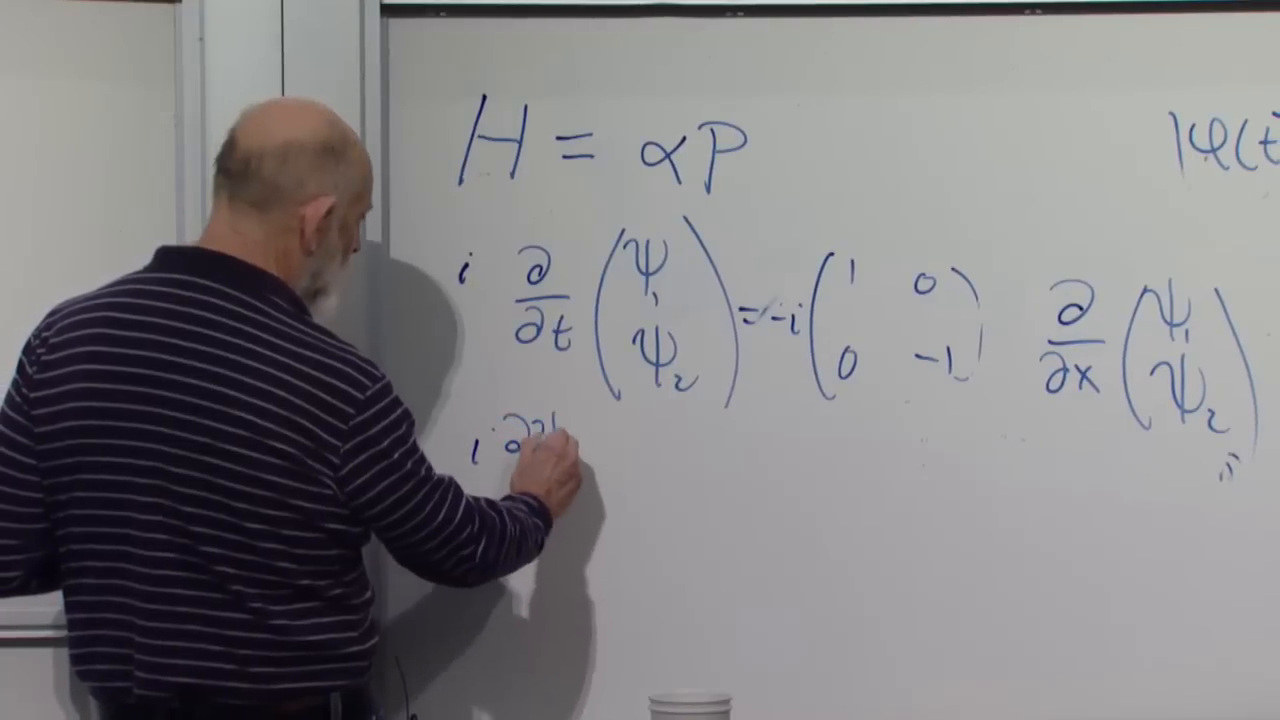
\includegraphics[width=0.94\linewidth]{lecture_09_frame_03.png}
\caption{Безмассовое двухкомпонентное уравнение на доске: \(H=\alpha P\), где диагональная матрица задаёт противоположные направления распространения для \(\psi_1\) и \(\psi_2\).}
\lectureframe{01:26:00}
\end{figure}

Проблема односторонности исчезла. Спектр с отрицательными энергиями остаётся, и мы обнаружили третий недостаток: обе компоненты по-прежнему безмассовы и распространяются со скоростью света. Следующий шаг должен ввести энергию покоя и связать эти направления.

\section{Добавление массы и открытие алгебры Дирака}

Добавим наиболее общий простой член, пропорциональный массе,
\begin{equation}
H=\alpha p+\beta m,
\label{eq:l9-dirac-hamiltonian}
\end{equation}
где \(\beta\) действует только на двухкомпонентный индекс. Это могла быть единичная матрица или какая-нибудь другая; предоставим выбор релятивистскому дисперсионному соотношению.

Поскольку \(H^2\) должно равняться \(p^2+m^2\), возведём в квадрат уравнение ~\eqref{eq:l9-dirac-hamiltonian}:
\begin{align}
H^2
&=(\alpha p+\beta m)^2\\
&=\alpha^2p^2+\beta^2m^2
+(\alpha\beta+\beta\alpha)pm.
\label{eq:l9-square-dirac}
\end{align}
Эти матрицы коммутируют с \(p\), потому что действуют во внутреннем двухкомпонентном пространстве, тогда как \(p\) действует на пространственную волновую функцию. Согласование с уравнением ~\eqref{eq:l9-rel-dispersion} требует
\begin{equation}
\alpha^2=\mathbb{1},
\qquad
\beta^2=\mathbb{1},
\qquad
\{\alpha,\beta\}
=\alpha\beta+\beta\alpha=0.
\label{eq:l9-dirac-algebra}
\end{equation}
Первое условие уже выполнено для \(\alpha=\sigma_3\). Любая другая матрица Паули антикоммутирует с ней и при возведении в квадрат даёт единичную матрицу. Выберем
\begin{equation}
\beta=
\begin{pmatrix}
0&1\\
1&0
\end{pmatrix}
=\sigma_1.
\label{eq:l9-beta}
\end{equation}
Выбор \(\sigma_1\) вместо \(\sigma_2\) — это вопрос соглашения о базисе; обе реализуют одну и ту же алгебру после унитарной замены базиса.

\begin{classroomqa}
\lecturetimestamp{01:33:00}
\audiencequestion{Неужели Дирак просто заметил, что матрицы Паули удовлетворяют этим алгебраическим условиям?}
\lecturerresponse{Исторически вывод сразу проводился в трёх измерениях и вводил матрицы, удовлетворяющие требуемым соотношениям. Как только условия записаны, алгебра Паули делает одномерное решение немедленным: достаточно выбрать две разные матрицы Паули.}
\end{classroomqa}

\begin{classroomqa}
\lecturetimestamp{01:34:24}
\audiencequestion{Является ли \(\beta\) релятивистским параметром скорости \(v/c\)?}
\lecturerresponse{Нет. Это матрица, действующая на компоненты спинора. Повторно используемая буква — всего лишь обозначение Дирака; она не имеет никакого отношения к кинематической величине \(v/c\).}
\end{classroomqa}

В трех пространственных измерениях матриц \(2\times2\) недостаточно для полного набора требуемых антикоммутирующих матриц. Это расширение отложено. В одном измерении уравнений~\eqref{eq:l9-alpha} и \eqref{eq:l9-beta} достаточно.

\section{Связанное одномерное уравнение Дирака}

Подстановка \(p=-i\partial_x\) дает одномерное уравнение Дирака в гамильтоновой форме:
\begin{equation}
i\partial_t\Psi
=\left(-i\alpha\partial_x+\beta m\right)\Psi.
\label{eq:l9-one-dimensional-dirac}
\end{equation}
Поскольку \(\alpha\) диагональна, ее член с производной оставляет две компоненты раздельными. Поскольку \(\beta\) внедиагональна, массовый член меняет их местами. Покомпонентно это записывается так:
\begin{align}
i\partial_t\psi_1
&=-i\partial_x\psi_1+m\psi_2,
\label{eq:l9-dirac-component-one}\\
i\partial_t\psi_2
&=+i\partial_x\psi_2+m\psi_1.
\label{eq:l9-dirac-component-two}
\end{align}

\begin{figure}[htbp]
\centering
\includegraphics[width=0.94\linewidth]{lecture_09_frame_08.png}
\caption{Связанные покомпонентные уравнения на доске. Противоположные знаки при производной кодируют движение вправо и влево; внедиагональный массовый член меняет местами \(\psi_1\) и \(\psi_2\).}
\lectureframe{01:37:44}
\end{figure}

Компоненты перестают эволюционировать независимо, как только \(m\ne0\). Возведение уравнения первого порядка в квадрат восстанавливает оператор Klein--Gordon для каждой компоненты,
\begin{equation}
\left(\partial_t^2-\partial_x^2+m^2\right)\psi_a=0,
\qquad a=1,2,
\end{equation}
а плоские волны удовлетворяют \(E^2=p^2+m^2\). Их групповая скорость равна
\begin{equation}
v_g=\frac{dE}{dp}=\frac{p}{E},
\end{equation}
модуль которой меньше единицы при ненулевой массе.

Связь между массой и смешением правого и левого секторов не случайна. Безмассовое праводвижущееся состояние остается праводвижущимся при любом собственном бусте Лоренца; никакой досветовой наблюдатель не может обогнать свет и обратить его направление. Массивную частицу можно привести в состояние покоя, а затем рассматривать из более быстрой системы отсчета, движущейся в том же направлении, где ее скорость кажется обращенной. Поэтому массивная релятивистская теория не может сохранять правый и левый секторы постоянно изолированными. Внедиагональный массовый член как раз и обеспечивает требуемую связь.

\begin{classroomqa}
\lecturetimestamp{01:40:01}
\audiencequestion{Является ли перестановка двух компонент хиральной осцилляцией?}
\lecturerresponse{В этом одномерном базисе \(\alpha\) различает два безмассовых хиральных направления. Массовый член внедиагонален и смешивает их, так что хиральность больше не сохраняется. В этом смысле массовый член является источником хиральной осцилляции.}
\end{classroomqa}

\begin{classroomqa}
\lecturetimestamp{01:40:46}
\audiencequestion{Почему уравнение фермиона должно быть квадратным корнем из уравнения бозона?}
\lecturerresponse{Так понимать это не следует. Дисперсионное соотношение \(E^2=p^2+m^2\) применимо к любой свободной релятивистской частице, независимо от статистики. Оператор Дирака просто дает матричную факторизацию оператора Klein--Gordon, но это алгебраическое соотношение не выводит фермионы из бозонов.}
\end{classroomqa}

\begin{classroomqa}
\lecturetimestamp{01:41:31}
\audiencequestion{Можно ли свести уравнение к простой скалярной факторизации на отдельные леводвижущиеся и праводвижущиеся множители?}
\lecturerresponse{Только в безмассовом пределе два хиральных уравнения расцепляются на независимые скалярные множители. При \(m\ne0\) полезна матричная факторизация: именно антикоммутирующие матрицы \(\alpha\) и \(\beta\) устраняют нежелательный перекрестный член.}
\end{classroomqa}

\begin{classroomqa}
\lecturetimestamp{01:42:04}
\audiencequestion{Составляют ли эти два связанных уравнения уже уравнение Дирака?}
\lecturerresponse{Да. Вместе они образуют уравнение Дирака в одном пространственном измерении; эквивалентно, оно записывается в компактной форме уравнения~\eqref{eq:l9-one-dimensional-dirac}. Более симметричную ковариантную запись можно получить, умножив на \(\beta\), но рассмотрение этой формы отложено.}
\end{classroomqa}

Две задачи намеренно оставлены незавершенными. Эта конструкция не устранила отрицательные энергии; она дала решения с отрицательной энергией в обоих секторах направлений движения, так что теперь эта проблема стала скорее более заметной, а не менее. Теория по-прежнему ограничена одним пространственным измерением. Следующие шаги — интерпретация решений с отрицательной энергией и расширение матричной алгебры до \(3+1\) измерений.
